% Created by tikzDevice version 0.12.3.1 on 2021-05-03 23:03:23
% !TEX encoding = UTF-8 Unicode
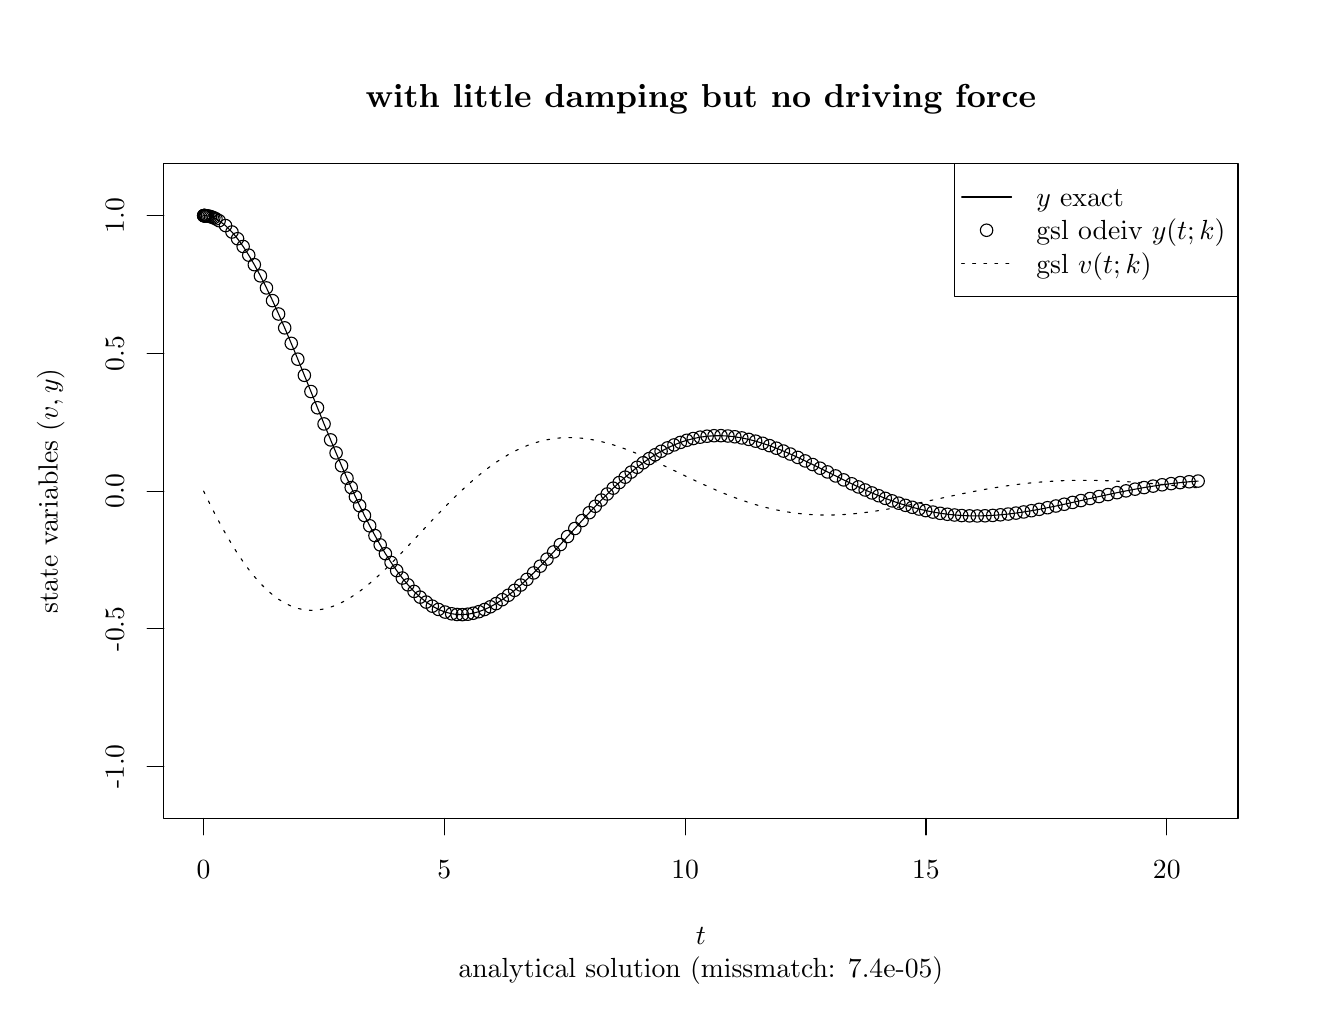
\begin{tikzpicture}[x=1pt,y=1pt]
\definecolor{fillColor}{RGB}{255,255,255}
\path[use as bounding box,fill=fillColor,fill opacity=0.00] (0,0) rectangle (462.53,346.90);
\begin{scope}
\path[clip] ( 49.20, 61.20) rectangle (437.33,297.70);
\definecolor{drawColor}{RGB}{0,0,0}

\path[draw=drawColor,line width= 0.4pt,line join=round,line cap=round] ( 63.58,278.98) --
	( 63.62,278.98) --
	( 63.69,278.98) --
	( 63.76,278.98) --
	( 63.82,278.98) --
	( 63.89,278.98) --
	( 63.96,278.97) --
	( 64.03,278.97) --
	( 64.12,278.97) --
	( 64.27,278.95) --
	( 64.53,278.93) --
	( 64.95,278.87) --
	( 65.52,278.76) --
	( 66.09,278.61) --
	( 66.66,278.42) --
	( 67.27,278.18) --
	( 68.04,277.81) --
	( 69.18,277.15) --
	( 71.50,275.38) --
	( 73.82,273.06) --
	( 75.84,270.63) --
	( 77.86,267.83) --
	( 79.88,264.70) --
	( 81.90,261.25) --
	( 84.10,257.21) --
	( 86.29,252.86) --
	( 88.48,248.26) --
	( 90.67,243.43) --
	( 92.87,238.42) --
	( 95.24,232.83) --
	( 97.61,227.10) --
	( 99.98,221.28) --
	(102.35,215.42) --
	(104.72,209.55) --
	(107.10,203.71) --
	(109.47,197.95) --
	(111.44,193.24) --
	(113.41,188.62) --
	(115.38,184.11) --
	(116.91,180.72) --
	(118.43,177.40) --
	(119.96,174.18) --
	(121.70,170.63) --
	(123.59,166.91) --
	(125.49,163.37) --
	(127.38,160.01) --
	(129.27,156.84) --
	(131.31,153.67) --
	(133.34,150.73) --
	(135.37,148.03) --
	(137.40,145.58) --
	(139.61,143.20) --
	(141.81,141.13) --
	(144.02,139.35) --
	(146.22,137.88) --
	(148.43,136.69) --
	(150.82,135.74) --
	(153.21,135.12) --
	(155.15,134.86) --
	(157.08,134.81) --
	(159.02,134.96) --
	(160.96,135.31) --
	(163.03,135.88) --
	(165.10,136.66) --
	(167.18,137.63) --
	(169.25,138.78) --
	(171.48,140.21) --
	(173.71,141.81) --
	(175.94,143.58) --
	(178.17,145.49) --
	(180.40,147.54) --
	(182.82,149.87) --
	(185.23,152.32) --
	(187.65,154.85) --
	(190.06,157.46) --
	(192.48,160.11) --
	(195.09,163.00) --
	(197.71,165.90) --
	(200.32,168.79) --
	(202.94,171.63) --
	(205.10,173.93) --
	(207.26,176.19) --
	(209.42,178.37) --
	(211.58,180.49) --
	(213.75,182.52) --
	(215.91,184.46) --
	(218.07,186.30) --
	(220.23,188.03) --
	(222.40,189.66) --
	(224.56,191.16) --
	(226.72,192.55) --
	(228.88,193.81) --
	(231.21,195.03) --
	(233.53,196.10) --
	(235.85,197.02) --
	(238.18,197.79) --
	(240.50,198.41) --
	(243.01,198.92) --
	(245.51,199.26) --
	(248.02,199.44) --
	(250.52,199.46) --
	(253.03,199.33) --
	(255.53,199.06) --
	(258.04,198.65) --
	(260.55,198.12) --
	(263.05,197.47) --
	(265.56,196.72) --
	(268.06,195.86) --
	(270.57,194.92) --
	(273.07,193.91) --
	(275.58,192.83) --
	(278.27,191.61) --
	(280.95,190.34) --
	(283.64,189.04) --
	(286.33,187.72) --
	(289.01,186.38) --
	(291.93,184.93) --
	(294.84,183.50) --
	(297.76,182.09) --
	(300.19,180.95) --
	(302.62,179.85) --
	(305.05,178.79) --
	(307.48,177.78) --
	(309.91,176.82) --
	(312.34,175.92) --
	(314.77,175.08) --
	(317.20,174.31) --
	(319.63,173.60) --
	(322.07,172.97) --
	(324.50,172.40) --
	(327.10,171.88) --
	(329.71,171.44) --
	(332.31,171.08) --
	(334.91,170.81) --
	(337.52,170.62) --
	(340.32,170.50) --
	(343.12,170.47) --
	(345.91,170.53) --
	(348.71,170.66) --
	(351.51,170.87) --
	(354.31,171.15) --
	(357.11,171.50) --
	(359.90,171.90) --
	(362.70,172.35) --
	(365.50,172.85) --
	(368.52,173.43) --
	(371.54,174.04) --
	(374.56,174.69) --
	(377.58,175.35) --
	(380.60,176.02) --
	(383.86,176.75) --
	(387.11,177.47) --
	(390.37,178.17) --
	(393.63,178.86) --
	(396.89,179.51) --
	(400.15,180.13) --
	(403.40,180.71) --
	(406.66,181.23) --
	(409.92,181.71) --
	(413.18,182.13) --
	(416.44,182.50) --
	(419.69,182.81) --
	(422.95,183.06);
\end{scope}
\begin{scope}
\path[clip] (  0.00,  0.00) rectangle (462.53,346.90);
\definecolor{drawColor}{RGB}{0,0,0}

\path[draw=drawColor,line width= 0.4pt,line join=round,line cap=round] ( 63.58, 61.20) -- (411.61, 61.20);

\path[draw=drawColor,line width= 0.4pt,line join=round,line cap=round] ( 63.58, 61.20) -- ( 63.58, 55.20);

\path[draw=drawColor,line width= 0.4pt,line join=round,line cap=round] (150.58, 61.20) -- (150.58, 55.20);

\path[draw=drawColor,line width= 0.4pt,line join=round,line cap=round] (237.59, 61.20) -- (237.59, 55.20);

\path[draw=drawColor,line width= 0.4pt,line join=round,line cap=round] (324.60, 61.20) -- (324.60, 55.20);

\path[draw=drawColor,line width= 0.4pt,line join=round,line cap=round] (411.61, 61.20) -- (411.61, 55.20);

\node[text=drawColor,anchor=base,inner sep=0pt, outer sep=0pt, scale=  1.00] at ( 63.58, 39.60) {0};

\node[text=drawColor,anchor=base,inner sep=0pt, outer sep=0pt, scale=  1.00] at (150.58, 39.60) {5};

\node[text=drawColor,anchor=base,inner sep=0pt, outer sep=0pt, scale=  1.00] at (237.59, 39.60) {10};

\node[text=drawColor,anchor=base,inner sep=0pt, outer sep=0pt, scale=  1.00] at (324.60, 39.60) {15};

\node[text=drawColor,anchor=base,inner sep=0pt, outer sep=0pt, scale=  1.00] at (411.61, 39.60) {20};

\path[draw=drawColor,line width= 0.4pt,line join=round,line cap=round] ( 49.20, 79.91) -- ( 49.20,278.98);

\path[draw=drawColor,line width= 0.4pt,line join=round,line cap=round] ( 49.20, 79.91) -- ( 43.20, 79.91);

\path[draw=drawColor,line width= 0.4pt,line join=round,line cap=round] ( 49.20,129.68) -- ( 43.20,129.68);

\path[draw=drawColor,line width= 0.4pt,line join=round,line cap=round] ( 49.20,179.45) -- ( 43.20,179.45);

\path[draw=drawColor,line width= 0.4pt,line join=round,line cap=round] ( 49.20,229.22) -- ( 43.20,229.22);

\path[draw=drawColor,line width= 0.4pt,line join=round,line cap=round] ( 49.20,278.98) -- ( 43.20,278.98);

\node[text=drawColor,rotate= 90.00,anchor=base,inner sep=0pt, outer sep=0pt, scale=  1.00] at ( 34.80, 79.91) {-1.0};

\node[text=drawColor,rotate= 90.00,anchor=base,inner sep=0pt, outer sep=0pt, scale=  1.00] at ( 34.80,129.68) {-0.5};

\node[text=drawColor,rotate= 90.00,anchor=base,inner sep=0pt, outer sep=0pt, scale=  1.00] at ( 34.80,179.45) {0.0};

\node[text=drawColor,rotate= 90.00,anchor=base,inner sep=0pt, outer sep=0pt, scale=  1.00] at ( 34.80,229.22) {0.5};

\node[text=drawColor,rotate= 90.00,anchor=base,inner sep=0pt, outer sep=0pt, scale=  1.00] at ( 34.80,278.98) {1.0};

\path[draw=drawColor,line width= 0.4pt,line join=round,line cap=round] ( 49.20, 61.20) --
	(437.33, 61.20) --
	(437.33,297.70) --
	( 49.20,297.70) --
	( 49.20, 61.20);
\end{scope}
\begin{scope}
\path[clip] (  0.00,  0.00) rectangle (462.53,346.90);
\definecolor{drawColor}{RGB}{0,0,0}

\node[text=drawColor,anchor=base,inner sep=0pt, outer sep=0pt, scale=  1.20] at (243.26,318.16) {\bfseries  with little damping but no driving force};

\node[text=drawColor,anchor=base,inner sep=0pt, outer sep=0pt, scale=  1.00] at (243.26,  3.60) {analytical solution (missmatch: 7.4e-05)};

\node[text=drawColor,anchor=base,inner sep=0pt, outer sep=0pt, scale=  1.00] at (243.26, 15.60) {$t$};

\node[text=drawColor,rotate= 90.00,anchor=base,inner sep=0pt, outer sep=0pt, scale=  1.00] at ( 10.80,179.45) {state variables $(v,y)$};
\end{scope}
\begin{scope}
\path[clip] ( 49.20, 61.20) rectangle (437.33,297.70);
\definecolor{drawColor}{RGB}{0,0,0}

\path[draw=drawColor,line width= 0.4pt,line join=round,line cap=round] ( 63.58,278.98) circle (  2.25);

\path[draw=drawColor,line width= 0.4pt,line join=round,line cap=round] ( 63.62,278.98) circle (  2.25);

\path[draw=drawColor,line width= 0.4pt,line join=round,line cap=round] ( 63.69,278.98) circle (  2.25);

\path[draw=drawColor,line width= 0.4pt,line join=round,line cap=round] ( 63.76,278.98) circle (  2.25);

\path[draw=drawColor,line width= 0.4pt,line join=round,line cap=round] ( 63.82,278.98) circle (  2.25);

\path[draw=drawColor,line width= 0.4pt,line join=round,line cap=round] ( 63.89,278.98) circle (  2.25);

\path[draw=drawColor,line width= 0.4pt,line join=round,line cap=round] ( 63.96,278.97) circle (  2.25);

\path[draw=drawColor,line width= 0.4pt,line join=round,line cap=round] ( 64.03,278.97) circle (  2.25);

\path[draw=drawColor,line width= 0.4pt,line join=round,line cap=round] ( 64.12,278.96) circle (  2.25);

\path[draw=drawColor,line width= 0.4pt,line join=round,line cap=round] ( 64.27,278.95) circle (  2.25);

\path[draw=drawColor,line width= 0.4pt,line join=round,line cap=round] ( 64.53,278.93) circle (  2.25);

\path[draw=drawColor,line width= 0.4pt,line join=round,line cap=round] ( 64.95,278.87) circle (  2.25);

\path[draw=drawColor,line width= 0.4pt,line join=round,line cap=round] ( 65.52,278.76) circle (  2.25);

\path[draw=drawColor,line width= 0.4pt,line join=round,line cap=round] ( 66.09,278.61) circle (  2.25);

\path[draw=drawColor,line width= 0.4pt,line join=round,line cap=round] ( 66.66,278.42) circle (  2.25);

\path[draw=drawColor,line width= 0.4pt,line join=round,line cap=round] ( 67.27,278.18) circle (  2.25);

\path[draw=drawColor,line width= 0.4pt,line join=round,line cap=round] ( 68.04,277.81) circle (  2.25);

\path[draw=drawColor,line width= 0.4pt,line join=round,line cap=round] ( 69.18,277.15) circle (  2.25);

\path[draw=drawColor,line width= 0.4pt,line join=round,line cap=round] ( 71.50,275.38) circle (  2.25);

\path[draw=drawColor,line width= 0.4pt,line join=round,line cap=round] ( 73.82,273.06) circle (  2.25);

\path[draw=drawColor,line width= 0.4pt,line join=round,line cap=round] ( 75.84,270.63) circle (  2.25);

\path[draw=drawColor,line width= 0.4pt,line join=round,line cap=round] ( 77.86,267.83) circle (  2.25);

\path[draw=drawColor,line width= 0.4pt,line join=round,line cap=round] ( 79.88,264.70) circle (  2.25);

\path[draw=drawColor,line width= 0.4pt,line join=round,line cap=round] ( 81.90,261.26) circle (  2.25);

\path[draw=drawColor,line width= 0.4pt,line join=round,line cap=round] ( 84.10,257.21) circle (  2.25);

\path[draw=drawColor,line width= 0.4pt,line join=round,line cap=round] ( 86.29,252.86) circle (  2.25);

\path[draw=drawColor,line width= 0.4pt,line join=round,line cap=round] ( 88.48,248.26) circle (  2.25);

\path[draw=drawColor,line width= 0.4pt,line join=round,line cap=round] ( 90.67,243.43) circle (  2.25);

\path[draw=drawColor,line width= 0.4pt,line join=round,line cap=round] ( 92.87,238.42) circle (  2.25);

\path[draw=drawColor,line width= 0.4pt,line join=round,line cap=round] ( 95.24,232.83) circle (  2.25);

\path[draw=drawColor,line width= 0.4pt,line join=round,line cap=round] ( 97.61,227.10) circle (  2.25);

\path[draw=drawColor,line width= 0.4pt,line join=round,line cap=round] ( 99.98,221.28) circle (  2.25);

\path[draw=drawColor,line width= 0.4pt,line join=round,line cap=round] (102.35,215.42) circle (  2.25);

\path[draw=drawColor,line width= 0.4pt,line join=round,line cap=round] (104.72,209.55) circle (  2.25);

\path[draw=drawColor,line width= 0.4pt,line join=round,line cap=round] (107.10,203.71) circle (  2.25);

\path[draw=drawColor,line width= 0.4pt,line join=round,line cap=round] (109.47,197.94) circle (  2.25);

\path[draw=drawColor,line width= 0.4pt,line join=round,line cap=round] (111.44,193.23) circle (  2.25);

\path[draw=drawColor,line width= 0.4pt,line join=round,line cap=round] (113.41,188.61) circle (  2.25);

\path[draw=drawColor,line width= 0.4pt,line join=round,line cap=round] (115.38,184.11) circle (  2.25);

\path[draw=drawColor,line width= 0.4pt,line join=round,line cap=round] (116.91,180.71) circle (  2.25);

\path[draw=drawColor,line width= 0.4pt,line join=round,line cap=round] (118.43,177.39) circle (  2.25);

\path[draw=drawColor,line width= 0.4pt,line join=round,line cap=round] (119.96,174.17) circle (  2.25);

\path[draw=drawColor,line width= 0.4pt,line join=round,line cap=round] (121.70,170.62) circle (  2.25);

\path[draw=drawColor,line width= 0.4pt,line join=round,line cap=round] (123.59,166.90) circle (  2.25);

\path[draw=drawColor,line width= 0.4pt,line join=round,line cap=round] (125.49,163.36) circle (  2.25);

\path[draw=drawColor,line width= 0.4pt,line join=round,line cap=round] (127.38,160.00) circle (  2.25);

\path[draw=drawColor,line width= 0.4pt,line join=round,line cap=round] (129.27,156.83) circle (  2.25);

\path[draw=drawColor,line width= 0.4pt,line join=round,line cap=round] (131.31,153.65) circle (  2.25);

\path[draw=drawColor,line width= 0.4pt,line join=round,line cap=round] (133.34,150.71) circle (  2.25);

\path[draw=drawColor,line width= 0.4pt,line join=round,line cap=round] (135.37,148.02) circle (  2.25);

\path[draw=drawColor,line width= 0.4pt,line join=round,line cap=round] (137.40,145.57) circle (  2.25);

\path[draw=drawColor,line width= 0.4pt,line join=round,line cap=round] (139.61,143.19) circle (  2.25);

\path[draw=drawColor,line width= 0.4pt,line join=round,line cap=round] (141.81,141.12) circle (  2.25);

\path[draw=drawColor,line width= 0.4pt,line join=round,line cap=round] (144.02,139.34) circle (  2.25);

\path[draw=drawColor,line width= 0.4pt,line join=round,line cap=round] (146.22,137.86) circle (  2.25);

\path[draw=drawColor,line width= 0.4pt,line join=round,line cap=round] (148.43,136.68) circle (  2.25);

\path[draw=drawColor,line width= 0.4pt,line join=round,line cap=round] (150.82,135.73) circle (  2.25);

\path[draw=drawColor,line width= 0.4pt,line join=round,line cap=round] (153.21,135.11) circle (  2.25);

\path[draw=drawColor,line width= 0.4pt,line join=round,line cap=round] (155.15,134.85) circle (  2.25);

\path[draw=drawColor,line width= 0.4pt,line join=round,line cap=round] (157.08,134.80) circle (  2.25);

\path[draw=drawColor,line width= 0.4pt,line join=round,line cap=round] (159.02,134.95) circle (  2.25);

\path[draw=drawColor,line width= 0.4pt,line join=round,line cap=round] (160.96,135.30) circle (  2.25);

\path[draw=drawColor,line width= 0.4pt,line join=round,line cap=round] (163.03,135.87) circle (  2.25);

\path[draw=drawColor,line width= 0.4pt,line join=round,line cap=round] (165.10,136.65) circle (  2.25);

\path[draw=drawColor,line width= 0.4pt,line join=round,line cap=round] (167.18,137.63) circle (  2.25);

\path[draw=drawColor,line width= 0.4pt,line join=round,line cap=round] (169.25,138.78) circle (  2.25);

\path[draw=drawColor,line width= 0.4pt,line join=round,line cap=round] (171.48,140.20) circle (  2.25);

\path[draw=drawColor,line width= 0.4pt,line join=round,line cap=round] (173.71,141.81) circle (  2.25);

\path[draw=drawColor,line width= 0.4pt,line join=round,line cap=round] (175.94,143.58) circle (  2.25);

\path[draw=drawColor,line width= 0.4pt,line join=round,line cap=round] (178.17,145.49) circle (  2.25);

\path[draw=drawColor,line width= 0.4pt,line join=round,line cap=round] (180.40,147.53) circle (  2.25);

\path[draw=drawColor,line width= 0.4pt,line join=round,line cap=round] (182.82,149.87) circle (  2.25);

\path[draw=drawColor,line width= 0.4pt,line join=round,line cap=round] (185.23,152.32) circle (  2.25);

\path[draw=drawColor,line width= 0.4pt,line join=round,line cap=round] (187.65,154.86) circle (  2.25);

\path[draw=drawColor,line width= 0.4pt,line join=round,line cap=round] (190.06,157.46) circle (  2.25);

\path[draw=drawColor,line width= 0.4pt,line join=round,line cap=round] (192.48,160.11) circle (  2.25);

\path[draw=drawColor,line width= 0.4pt,line join=round,line cap=round] (195.09,163.01) circle (  2.25);

\path[draw=drawColor,line width= 0.4pt,line join=round,line cap=round] (197.71,165.91) circle (  2.25);

\path[draw=drawColor,line width= 0.4pt,line join=round,line cap=round] (200.32,168.79) circle (  2.25);

\path[draw=drawColor,line width= 0.4pt,line join=round,line cap=round] (202.94,171.64) circle (  2.25);

\path[draw=drawColor,line width= 0.4pt,line join=round,line cap=round] (205.10,173.95) circle (  2.25);

\path[draw=drawColor,line width= 0.4pt,line join=round,line cap=round] (207.26,176.20) circle (  2.25);

\path[draw=drawColor,line width= 0.4pt,line join=round,line cap=round] (209.42,178.39) circle (  2.25);

\path[draw=drawColor,line width= 0.4pt,line join=round,line cap=round] (211.58,180.50) circle (  2.25);

\path[draw=drawColor,line width= 0.4pt,line join=round,line cap=round] (213.75,182.53) circle (  2.25);

\path[draw=drawColor,line width= 0.4pt,line join=round,line cap=round] (215.91,184.47) circle (  2.25);

\path[draw=drawColor,line width= 0.4pt,line join=round,line cap=round] (218.07,186.31) circle (  2.25);

\path[draw=drawColor,line width= 0.4pt,line join=round,line cap=round] (220.23,188.05) circle (  2.25);

\path[draw=drawColor,line width= 0.4pt,line join=round,line cap=round] (222.40,189.67) circle (  2.25);

\path[draw=drawColor,line width= 0.4pt,line join=round,line cap=round] (224.56,191.18) circle (  2.25);

\path[draw=drawColor,line width= 0.4pt,line join=round,line cap=round] (226.72,192.57) circle (  2.25);

\path[draw=drawColor,line width= 0.4pt,line join=round,line cap=round] (228.88,193.83) circle (  2.25);

\path[draw=drawColor,line width= 0.4pt,line join=round,line cap=round] (231.21,195.05) circle (  2.25);

\path[draw=drawColor,line width= 0.4pt,line join=round,line cap=round] (233.53,196.11) circle (  2.25);

\path[draw=drawColor,line width= 0.4pt,line join=round,line cap=round] (235.85,197.03) circle (  2.25);

\path[draw=drawColor,line width= 0.4pt,line join=round,line cap=round] (238.18,197.80) circle (  2.25);

\path[draw=drawColor,line width= 0.4pt,line join=round,line cap=round] (240.50,198.43) circle (  2.25);

\path[draw=drawColor,line width= 0.4pt,line join=round,line cap=round] (243.01,198.93) circle (  2.25);

\path[draw=drawColor,line width= 0.4pt,line join=round,line cap=round] (245.51,199.27) circle (  2.25);

\path[draw=drawColor,line width= 0.4pt,line join=round,line cap=round] (248.02,199.45) circle (  2.25);

\path[draw=drawColor,line width= 0.4pt,line join=round,line cap=round] (250.52,199.47) circle (  2.25);

\path[draw=drawColor,line width= 0.4pt,line join=round,line cap=round] (253.03,199.34) circle (  2.25);

\path[draw=drawColor,line width= 0.4pt,line join=round,line cap=round] (255.53,199.07) circle (  2.25);

\path[draw=drawColor,line width= 0.4pt,line join=round,line cap=round] (258.04,198.66) circle (  2.25);

\path[draw=drawColor,line width= 0.4pt,line join=round,line cap=round] (260.55,198.13) circle (  2.25);

\path[draw=drawColor,line width= 0.4pt,line join=round,line cap=round] (263.05,197.48) circle (  2.25);

\path[draw=drawColor,line width= 0.4pt,line join=round,line cap=round] (265.56,196.72) circle (  2.25);

\path[draw=drawColor,line width= 0.4pt,line join=round,line cap=round] (268.06,195.87) circle (  2.25);

\path[draw=drawColor,line width= 0.4pt,line join=round,line cap=round] (270.57,194.93) circle (  2.25);

\path[draw=drawColor,line width= 0.4pt,line join=round,line cap=round] (273.07,193.91) circle (  2.25);

\path[draw=drawColor,line width= 0.4pt,line join=round,line cap=round] (275.58,192.83) circle (  2.25);

\path[draw=drawColor,line width= 0.4pt,line join=round,line cap=round] (278.27,191.61) circle (  2.25);

\path[draw=drawColor,line width= 0.4pt,line join=round,line cap=round] (280.95,190.34) circle (  2.25);

\path[draw=drawColor,line width= 0.4pt,line join=round,line cap=round] (283.64,189.04) circle (  2.25);

\path[draw=drawColor,line width= 0.4pt,line join=round,line cap=round] (286.33,187.71) circle (  2.25);

\path[draw=drawColor,line width= 0.4pt,line join=round,line cap=round] (289.01,186.37) circle (  2.25);

\path[draw=drawColor,line width= 0.4pt,line join=round,line cap=round] (291.93,184.92) circle (  2.25);

\path[draw=drawColor,line width= 0.4pt,line join=round,line cap=round] (294.84,183.49) circle (  2.25);

\path[draw=drawColor,line width= 0.4pt,line join=round,line cap=round] (297.76,182.08) circle (  2.25);

\path[draw=drawColor,line width= 0.4pt,line join=round,line cap=round] (300.19,180.94) circle (  2.25);

\path[draw=drawColor,line width= 0.4pt,line join=round,line cap=round] (302.62,179.84) circle (  2.25);

\path[draw=drawColor,line width= 0.4pt,line join=round,line cap=round] (305.05,178.78) circle (  2.25);

\path[draw=drawColor,line width= 0.4pt,line join=round,line cap=round] (307.48,177.77) circle (  2.25);

\path[draw=drawColor,line width= 0.4pt,line join=round,line cap=round] (309.91,176.81) circle (  2.25);

\path[draw=drawColor,line width= 0.4pt,line join=round,line cap=round] (312.34,175.91) circle (  2.25);

\path[draw=drawColor,line width= 0.4pt,line join=round,line cap=round] (314.77,175.07) circle (  2.25);

\path[draw=drawColor,line width= 0.4pt,line join=round,line cap=round] (317.20,174.29) circle (  2.25);

\path[draw=drawColor,line width= 0.4pt,line join=round,line cap=round] (319.63,173.59) circle (  2.25);

\path[draw=drawColor,line width= 0.4pt,line join=round,line cap=round] (322.07,172.95) circle (  2.25);

\path[draw=drawColor,line width= 0.4pt,line join=round,line cap=round] (324.50,172.39) circle (  2.25);

\path[draw=drawColor,line width= 0.4pt,line join=round,line cap=round] (327.10,171.86) circle (  2.25);

\path[draw=drawColor,line width= 0.4pt,line join=round,line cap=round] (329.71,171.42) circle (  2.25);

\path[draw=drawColor,line width= 0.4pt,line join=round,line cap=round] (332.31,171.07) circle (  2.25);

\path[draw=drawColor,line width= 0.4pt,line join=round,line cap=round] (334.91,170.80) circle (  2.25);

\path[draw=drawColor,line width= 0.4pt,line join=round,line cap=round] (337.52,170.60) circle (  2.25);

\path[draw=drawColor,line width= 0.4pt,line join=round,line cap=round] (340.32,170.49) circle (  2.25);

\path[draw=drawColor,line width= 0.4pt,line join=round,line cap=round] (343.12,170.46) circle (  2.25);

\path[draw=drawColor,line width= 0.4pt,line join=round,line cap=round] (345.91,170.52) circle (  2.25);

\path[draw=drawColor,line width= 0.4pt,line join=round,line cap=round] (348.71,170.65) circle (  2.25);

\path[draw=drawColor,line width= 0.4pt,line join=round,line cap=round] (351.51,170.87) circle (  2.25);

\path[draw=drawColor,line width= 0.4pt,line join=round,line cap=round] (354.31,171.15) circle (  2.25);

\path[draw=drawColor,line width= 0.4pt,line join=round,line cap=round] (357.11,171.49) circle (  2.25);

\path[draw=drawColor,line width= 0.4pt,line join=round,line cap=round] (359.90,171.90) circle (  2.25);

\path[draw=drawColor,line width= 0.4pt,line join=round,line cap=round] (362.70,172.35) circle (  2.25);

\path[draw=drawColor,line width= 0.4pt,line join=round,line cap=round] (365.50,172.85) circle (  2.25);

\path[draw=drawColor,line width= 0.4pt,line join=round,line cap=round] (368.52,173.43) circle (  2.25);

\path[draw=drawColor,line width= 0.4pt,line join=round,line cap=round] (371.54,174.05) circle (  2.25);

\path[draw=drawColor,line width= 0.4pt,line join=round,line cap=round] (374.56,174.69) circle (  2.25);

\path[draw=drawColor,line width= 0.4pt,line join=round,line cap=round] (377.58,175.35) circle (  2.25);

\path[draw=drawColor,line width= 0.4pt,line join=round,line cap=round] (380.60,176.02) circle (  2.25);

\path[draw=drawColor,line width= 0.4pt,line join=round,line cap=round] (383.86,176.75) circle (  2.25);

\path[draw=drawColor,line width= 0.4pt,line join=round,line cap=round] (387.11,177.47) circle (  2.25);

\path[draw=drawColor,line width= 0.4pt,line join=round,line cap=round] (390.37,178.18) circle (  2.25);

\path[draw=drawColor,line width= 0.4pt,line join=round,line cap=round] (393.63,178.87) circle (  2.25);

\path[draw=drawColor,line width= 0.4pt,line join=round,line cap=round] (396.89,179.52) circle (  2.25);

\path[draw=drawColor,line width= 0.4pt,line join=round,line cap=round] (400.15,180.14) circle (  2.25);

\path[draw=drawColor,line width= 0.4pt,line join=round,line cap=round] (403.40,180.72) circle (  2.25);

\path[draw=drawColor,line width= 0.4pt,line join=round,line cap=round] (406.66,181.24) circle (  2.25);

\path[draw=drawColor,line width= 0.4pt,line join=round,line cap=round] (409.92,181.72) circle (  2.25);

\path[draw=drawColor,line width= 0.4pt,line join=round,line cap=round] (413.18,182.14) circle (  2.25);

\path[draw=drawColor,line width= 0.4pt,line join=round,line cap=round] (416.44,182.51) circle (  2.25);

\path[draw=drawColor,line width= 0.4pt,line join=round,line cap=round] (419.69,182.82) circle (  2.25);

\path[draw=drawColor,line width= 0.4pt,line join=round,line cap=round] (422.95,183.07) circle (  2.25);

\path[draw=drawColor,line width= 0.4pt,dash pattern=on 1pt off 3pt ,line join=round,line cap=round] ( 63.58,179.45) --
	( 63.62,179.35) --
	( 63.69,179.21) --
	( 63.76,179.07) --
	( 63.82,178.92) --
	( 63.89,178.78) --
	( 63.96,178.64) --
	( 64.03,178.51) --
	( 64.12,178.31) --
	( 64.27,177.99) --
	( 64.53,177.45) --
	( 64.95,176.60) --
	( 65.52,175.43) --
	( 66.09,174.28) --
	( 66.66,173.15) --
	( 67.27,171.94) --
	( 68.04,170.45) --
	( 69.18,168.29) --
	( 71.50,164.07) --
	( 73.82,160.11) --
	( 75.84,156.89) --
	( 77.86,153.89) --
	( 79.88,151.12) --
	( 81.90,148.58) --
	( 84.10,146.09) --
	( 86.29,143.89) --
	( 88.48,141.98) --
	( 90.67,140.35) --
	( 92.87,139.00) --
	( 95.24,137.86) --
	( 97.61,137.04) --
	( 99.98,136.55) --
	(102.35,136.35) --
	(104.72,136.46) --
	(107.10,136.85) --
	(109.47,137.50) --
	(111.44,138.24) --
	(113.41,139.15) --
	(115.38,140.22) --
	(116.91,141.14) --
	(118.43,142.15) --
	(119.96,143.23) --
	(121.70,144.56) --
	(123.59,146.10) --
	(125.49,147.74) --
	(127.38,149.46) --
	(129.27,151.25) --
	(131.31,153.24) --
	(133.34,155.30) --
	(135.37,157.40) --
	(137.40,159.54) --
	(139.61,161.89) --
	(141.81,164.25) --
	(144.02,166.61) --
	(146.22,168.96) --
	(148.43,171.28) --
	(150.82,173.75) --
	(153.21,176.17) --
	(155.15,178.07) --
	(157.08,179.91) --
	(159.02,181.69) --
	(160.96,183.40) --
	(163.03,185.15) --
	(165.10,186.81) --
	(167.18,188.38) --
	(169.25,189.84) --
	(171.48,191.30) --
	(173.71,192.63) --
	(175.94,193.83) --
	(178.17,194.91) --
	(180.40,195.85) --
	(182.82,196.72) --
	(185.23,197.43) --
	(187.65,197.99) --
	(190.06,198.40) --
	(192.48,198.66) --
	(195.09,198.78) --
	(197.71,198.74) --
	(200.32,198.54) --
	(202.94,198.20) --
	(205.10,197.81) --
	(207.26,197.33) --
	(209.42,196.77) --
	(211.58,196.14) --
	(213.75,195.44) --
	(215.91,194.67) --
	(218.07,193.84) --
	(220.23,192.97) --
	(222.40,192.05) --
	(224.56,191.10) --
	(226.72,190.11) --
	(228.88,189.11) --
	(231.21,188.00) --
	(233.53,186.89) --
	(235.85,185.77) --
	(238.18,184.66) --
	(240.50,183.55) --
	(243.01,182.38) --
	(245.51,181.24) --
	(248.02,180.13) --
	(250.52,179.06) --
	(253.03,178.04) --
	(255.53,177.08) --
	(258.04,176.17) --
	(260.55,175.33) --
	(263.05,174.55) --
	(265.56,173.84) --
	(268.06,173.20) --
	(270.57,172.64) --
	(273.07,172.15) --
	(275.58,171.74) --
	(278.27,171.38) --
	(280.95,171.10) --
	(283.64,170.91) --
	(286.33,170.80) --
	(289.01,170.77) --
	(291.93,170.83) --
	(294.84,170.96) --
	(297.76,171.18) --
	(300.19,171.41) --
	(302.62,171.70) --
	(305.05,172.02) --
	(307.48,172.39) --
	(309.91,172.79) --
	(312.34,173.21) --
	(314.77,173.67) --
	(317.20,174.15) --
	(319.63,174.64) --
	(322.07,175.15) --
	(324.50,175.67) --
	(327.10,176.23) --
	(329.71,176.79) --
	(332.31,177.35) --
	(334.91,177.90) --
	(337.52,178.44) --
	(340.32,179.00) --
	(343.12,179.54) --
	(345.91,180.06) --
	(348.71,180.54) --
	(351.51,180.99) --
	(354.31,181.41) --
	(357.11,181.78) --
	(359.90,182.12) --
	(362.70,182.42) --
	(365.50,182.67) --
	(368.52,182.90) --
	(371.54,183.08) --
	(374.56,183.22) --
	(377.58,183.30) --
	(380.60,183.34) --
	(383.86,183.33) --
	(387.11,183.27) --
	(390.37,183.17) --
	(393.63,183.03) --
	(396.89,182.85) --
	(400.15,182.64) --
	(403.40,182.40) --
	(406.66,182.14) --
	(409.92,181.85) --
	(413.18,181.55) --
	(416.44,181.25) --
	(419.69,180.93) --
	(422.95,180.62);
\definecolor{fillColor}{RGB}{255,255,255}

\path[draw=drawColor,line width= 0.4pt,line join=round,line cap=round,fill=fillColor] (334.80,297.70) rectangle (437.33,249.70);

\path[draw=drawColor,line width= 0.4pt,line join=round,line cap=round] (337.50,285.70) -- (355.50,285.70);

\path[draw=drawColor,line width= 0.4pt,dash pattern=on 1pt off 3pt ,line join=round,line cap=round] (337.50,261.70) -- (355.50,261.70);

\path[draw=drawColor,line width= 0.4pt,line join=round,line cap=round] (346.50,273.70) circle (  2.25);

\node[text=drawColor,anchor=base west,inner sep=0pt, outer sep=0pt, scale=  1.00] at (364.50,282.25) {$y$ exact};

\node[text=drawColor,anchor=base west,inner sep=0pt, outer sep=0pt, scale=  1.00] at (364.50,270.25) {gsl odeiv $y(t;k)$};

\node[text=drawColor,anchor=base west,inner sep=0pt, outer sep=0pt, scale=  1.00] at (364.50,258.25) {gsl $v(t;k)$};
\end{scope}
\end{tikzpicture}
